\chapter{Asymmetrische Verschlüsselung}
\label{ch:asymmenc}

Symmetrische Verschlüsselung, wie wir sie in den letzten Kapiteln
behandelt haben, funktioniert über ein gemeinsames Geheimnis $K$.  Das
verursacht uns einige Unannehmlichkeiten:

\begin{itemize}
\item das gemeinsame Geheimnis $K$ muss auf einem sicheren Kanal
  übertragen werden.
\item bei $n$ Benutzern werden im System $\binom{n}{2} = \frac{n \cdot
    (n-1)}{2}$ Schlüssel verwendet (für jedes Teilnehmerpaar einen).
\end{itemize}

\section{Idee} Asymmetrische Verschlüsselung\indexEncryptionAsymm, auch
\emph{Public-Key-Kryptographie} genannt, basiert auf der Grundidee, für
die Verschlüsselung (öffentlich) einen anderen Schlüssel zu verwenden
als für die Entschlüsselung (privat).

Die Vorteile eines Public-Key-Verfahrens sind offensichtlich. Wir
benötigen für den Schlüsselaustausch keinen sicheren Kanal mehr, sondern
könnten sogar ähnlich einem Telefonbuch ein öffentliches Verzeichnis mit
den öffentlichen Schlüsseln anlegen. Außerdem müssen nicht mehr so viele
Schlüssel gespeichert werden: Bei $n$ Benutzern gibt es nur noch $n$
öffentliche (und $n$ geheime) Schlüssel.

Die Sicherheit eines solchen Verfahrens hängt davon ab, wie schwierig es
für einen Angreifer ist, vom (allgemein bekannten) öffentlichen
Schlüssel $pk$ auf den (geheim gehaltenen) privaten Schlüssel $sk$ zu
schließen. Um das praktisch unmöglich zu machen, greift man auf Probleme
zurück, die nach aktuellem Forschungsstand nicht effizient lösbar
sind. Im Folgenden werden zwei Verfahren vorgestellt, die asymmetrische
Verschlüsselung basierend auf dem RSA-Problem bzw. dem DLOG-Problem
konstruieren.

\begin{figure}
  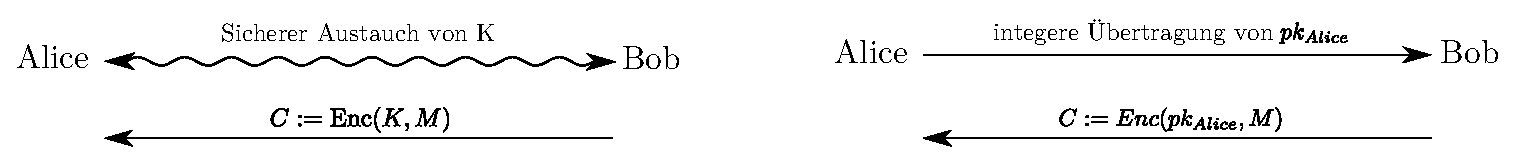
\includegraphics[width=\textwidth]{images/vergleich-symmetrisch-asymmetrisch.eps}
  \caption{Unterschiede in der Vorbereitung von symmetrisch und
    asymmetrisch verschlüsselter Kommunikation}
  \label{fig:asymmenc-symmenc}
\end{figure} Damit Bob eine asymmetrisch verschlüsselte Nachricht an
Alice senden kann, benötigt er ihren öffentlichen Schlüssel. Dieser darf
unverschlüsselt verschickt werden, es muss aber sichergestellt werden,
dass der Schlüssel nicht bei der Kommunikation manipuliert wurde. Dies
geschieht über eine sogenannte \textit{Public Key Infrastructure}, was
hier jedoch nicht weiter vertieft wird.
\section{Sicherheitsbegriffe für asymmetrische Verfahren} Die
Sicherheitsbegriffe, die wir in Kapitel \ref{chap:krypt-begriffe} kennen
gelernt haben, finden mit leicht abgewandelten Definitionen auch bei
asymmetrischen Verfahren Anwendung:

\begin{definition}[Semantische Sicherheit für Public-Key-Verfahren] Ein
  Pub\-lic-""Key-""Ver\-schlüs\-sel\-ungs\-sche\-ma ist \textit{semantisch
    sicher}, wenn es für jede $M$-Verteilung von Nachrichten gleicher Länge,
  jede Funktion $f$ und jeden PPT-Algorithmus $\A$ einen PPT-Algorithmus
  $\B$ gibt, so dass
  \begin{equation*} \Pr\left[\A(1^k, pk, \enc(pk, M)) = f(M)\right] -
    \Pr\left[\B(1^k) = f(M)\right]
  \end{equation*} vernachlässigbar (als Funktion im Sicherheitsparameter)
  ist.
\end{definition}

\begin{definition}[IND-CPA-Sicherheit für
  Public-Key-Verfahren]\indexINDCPA Betrachte folgendes Experiment mit
  einem Herausforderer $\C$ und einem PPT-Angreifer $\A$.
  \begin{itemize}
  \item $\C$ generiert mit dem Generator-Algorithmus ein Schlüsselpaar,
    d.h. er berechnet $(pk, sk)$.
  \item $\A$ erhält $pk$ und kann sich zu jedem Zeitpunkt jedes
    beliebige $\plaint$ mithilfe von $pk$ verschlüsseln.
  \end{itemize}
  \begin{enumerate}
  \item $\A$ wählt zwei Nachrichten $\plaint_1$, $\plaint_2$ gleicher
    Länge.
  \item $\A$ erhält $\ciphert^{*} := \enc(pk, \plaint_{b})$ für ein von
    $\C$ zufällig gleichverteilt gewähltes $b \in \{1, 2\}$.
  \item $\A$ gewinnt, wenn er $b$ korrekt errät.
  \end{enumerate} Ein asymmetrisches Verfahren $(\gen, \enc, \dec)$
  heißt IND-CPA-sicher, wenn der Vorteil des Angreifers gegenüber dem
  Raten einer Lösung, also $\Pr \left[ \A \textnormal{ gewinnt} \right] -
  \frac{1}{2}$, für alle PPT-Algorithmen $\A$ vernachlässigbar im
  Sicherheitsparameter $k$ ist.
\end{definition}

Der IND-CPA-Begriff unterscheidet sich also dadurch vom symmetrischen
Fall, dass ein Angreifer $\A$ kein Orakel mehr braucht, sondern
Chiffrate selbst mit dem öffentlichen Schlüssel erzeugen kann.

Auch IND-CCA hat eine Variante für asymmetrische Verfahren, die wir aber
nicht weiter vertiefen.


\section{RSA-Verschlüsselung} Das bekannteste Public-Key-Verfahren ist
RSA\indexRSATextBook (1977). Es ist benannt nach seinen Erfindern
Ronald Rivest, Adi Shamir und Leonard Adleman.

\subsection{Erweiterter Euklidischer Algorithmus}
\label{ssec:eea} Um das Vorgehen der Schlüsselerzeugung des
RSA-Algorithmus erklären zu können, führen wir den \emph{Erweiterten
  Euklidischen Algorithmus} (EEA)\indexEEA als Hilfskonstrukt ein, der es
uns erlaubt, das inverse Element $t$ zu $B$ über einer multiplikativen
Gruppe $\mathbbm{Z}^{\ast}_{A}$ zu bestimmen. Für gegebene Parameter $A$
und $B$ berechnet der EEA neben dem größten gemeinsamen Teiler $\ggT(A,
B)$ zwei ganze Zahlen $s$ und $t$, sodass

\begin{align*} \ggt(A, B) = s \cdot A + t \cdot B\, .
\end{align*}

Für das RSA-Verfahren reicht es, den Spezialfall $\ggT(A,B) = 1$ zu
betrachten, der folgenden Zusammenhang liefert:

\begin{align*} 1 &= s \cdot A + t \cdot B\\ \Leftrightarrow 1 &\equiv t
                                                                \cdot B \pmod A
\end{align*}

Bezüglich $\mathbbm{Z}^*_{A}$ ist $t$ also das zu $B$
multiplikativ-inverse Element. Das Vorgehen betrachten wir beispielhaft
für $B = 23$, zu dem das inverse Element über $\mathbbm{Z}^{\ast}_{192}$
bestimmt werden soll.

Wir betrachten im Folgenden zwei Varianten des erweiterten Euklidischen
Algorithmus.

Der EEA entwickelt zwei Variablen $s$ und $t$ iterativ, sodass gilt:
\begin{align*} s_{i+1} &= s_{i-1} - f_{i+1} \cdot s_{i}\\ t_{i+1} &=
                                                                    t_{i-1} - f_{i+1} \cdot t_{i}
\end{align*} Hierbei ist $f_i = \max \{f : f \cdot B_i \leq A_i\}$
und die größte Zahl, die $R_i > 0$
\begin{beispiel}[EEA] Es sei $A = A_2 = 192 $ und $B = B_2 = 23$. Es
  ist $\ggT(192, 23) = 1$, da B prim und A kein Vielfaches von B ist . Nun
  berechnen wir ausgehend von $i = 2$ in
  \begin{align*} A_i = f_i \cdot B_i + R_i
  \end{align*} jeweils $f_i = \max \{f : f \cdot B_i \leq A_i\}$ und
  $R_i > 0$, bis $R_i = 0$. Dabei ist $A_{i+1} = B_i$ und $B_{i+1} =
  R_i$. Parallel dazu entwickeln wir die Parameter $s$ und $t$ über die
  Gleichungen \emph{vorwärts}. Wir erhalten demnach
  \begin{table}[h] \centering \large
    \begin{tabular}[c]{|c|l|rrr|l|} \hline & Gleichung & $R_i$ & $s_i$ & $t_i$ &\\ 
      \hline 
      \hline 
      (0) & $192 = 1 \cdot 192 + 0 \cdot 23$ & $192$ & $1$ & $0$ &\\
      (1) & $23 = 0 \cdot 192 + 1 \cdot 23$ & $23$ & $0$ & $1$   &\\ 
      \hline 
          & EEA & & & &\\ 
      \hline 
      (2) & $192 = 8 \cdot 23 + 8$ & $8$ & $1$ & $-8$ & $\text{(0)} - 8 \cdot\text{(1)}$\\
      (3) & $23 = 2 \cdot 8 + 7$ & $7$ & $-2$ & $17$ & $\text{(1)} - 2  \cdot \text{(2)}$\\ 
      (4) & $8 = 1 \cdot 7 + 1$ & $1$ & $3$ & $-25$ & $\text{(2)} - 1 \cdot \text{(3)}$\\
      (5) & $7 = 7 \cdot 1 + 0$ & $0$ & $-23$ & $192$ & $\text{(3)} - 7 \cdot\text{(4)}$\\ 
      \hline
    \end{tabular}
  \end{table}
  \subsubsection*{Varianten 1: Vorwärts-Entwicklung} Die vom EEA
  berechneten Werte, das heißt die Parameter $s$ und $t$, stehen in der
  (4). Zeile. Es ist also
  \begin{align*} 1    &= 3 \cdot 192 + (-25) \cdot 23\\ 
    \Leftrightarrow 1 &\equiv (-25) \cdot 23 \pmod{192}\\ 
    \Leftrightarrow 1 &\equiv (192 - 25)\cdot 23 \pmod{192}\\
    \Leftrightarrow 1 &\equiv 167 \cdot 23 \pmod{192}\, \text{,}
  \end{align*} 
  und somit $167$ das zu $23$ multiplikativ-inverse Element bezüglich
  $\mathbbm{Z}^{\ast}_{192}$.
  \subsubsection*{Varianten 2: Rückwärts-Entwicklung} 
  Ebenso ist es möglich, die Parameter $s$ und $t$ \emph{rückwärts} zu
  berechnen. Dazu werden, ausgehend von (2), die Gleichungen (3), (4) und
  (5) aufgestellt und anschließend wie folgt ineinander eingesetzt:
  \begin{align*}
    \begin{split}
      1 &\stackrel{\textit{(4)}}{=} 8 - 1 \cdot 7\\
        &\stackrel{\textit{(3)}}{=} 8 - 1 \cdot (23 - 2 \cdot 8) = -23 + 3 \cdot 8\\ 
        &\stackrel{\textit{(2)}}{=} -23 + 3 \cdot (192 - 8 \cdot 23) = 3\cdot 192 - 25 \cdot 23\\
 [.5cm] &\equiv -25 \cdot 23 \pmod{192}\\
        &\equiv 167 \cdot 23 \pmod{192}
    \end{split}
  \end{align*}
\end{beispiel}

\subsection{Vorgehen}
\label{ch:asymmenc:rsa:vorgehen} Um RSA\indexRSATextBook nutzen zu
können, brauchen wir drei Algorithmen: Einen Generator-Algorithmus
$\operatorname{Gen}$, einen Verschlüsselungsalgorithmus
$\operatorname{Enc}$ und einen Entschlüsselungsalgorithmus
$\operatorname{Dec}$.
\subsubsection{Generator-Algorithmus} Für die Erstellung eines
Schlüsselpaares werden zwei große Primzahlen benötigt. Die Berechnung
des öffentlichen und privaten Schlüssels funktioniert folgendermaßen:
\begin{itemize}
\item Wähle zwei große Primzahlen $P, Q$ mit $P \neq Q$ und
  vorgegebener Bitlänge $k$.
\item Berechne $N = P \cdot Q$.
\item Berechne $\varphi(N) = (P - 1)(Q - 1)$\footnote{$\varphi$
    bezeichnet die Eulersche Phi-Funktion\indexEulerPhiFunction. Sie gibt
    für jede natürliche Zahl n an, wie viele zu n teilerfremde natürliche
    Zahlen es gibt, die nicht größer als n sind: $\varphi(n) := \vert
    \{a\in\N \, |\, 1 \le a \le n \land \operatorname{ggT}(a,n) = 1 \}
    \vert$. Insbesondere ist $\varphi(N)$ die Anzahl multiplikativ
    invertierbarer Elemente im Restklassenring $\mathbb{Z}/N\mathbb{Z}$.
    Sie ist multiplikativ, d.h. es gilt für teilerfremde $n$, $m$:
    $\varphi(m\cdot n) = \varphi(m) \cdot \varphi(n)$. Da eine Primzahlen
    $p$ nur durch 1 und sich selbst teilbar ist, gilt $\varphi(p) =
    p-1$. Somit gilt für zwei Primzahlen $p$, $q$ also $\phi(p \cdot q) =
    \phi(p) \cdot \phi(q) = (p-1)(q-1)$.}.
\item Wähle $e \in \{3, \dotsc, \varphi(N) - 1\}$, wobei
  $\ggT(e, \varphi(N)) = 1$.
\item Berechne mit Hilfe des \hyperref[ssec:eea]{EEA} das zu $e$
  multiplikativ-inverse Element $d$ bezüglich $\varphi(N)$, d.h. $d \equiv
  e^{-1} \pmod{\varphi(N)}$.
\end{itemize}

Damit ist der geheime Schlüssel $sk = (N, d)$ und $pk = (N, e)$ der
öffentliche Schlüssel. Üblicherweise werden $P$ und $Q$ zufällig
gleichverteilt aus den ungeraden Zahlen der Bitlänge $k$ gezogen, bis
$P$ und $Q$ prim sind. Der Nachrichtenraum ist \Z{N}.
\subsubsection{Ver- und Entschlüsselung} Für die Ver- und
Entschlüsselungsfunktion gilt:
\begin{align*} \enc(pk, M) & = M^e \mod N \\ \dec(sk, C) & = C^d \mod N
\end{align*}

Wie immer muss $\dec(\enc(M)) = M$ gelten. Für die Korrektheit von RSA
bedeutet das, dass
\begin{align*} (M^e)^d \equiv M^{ed} \equiv M \pmod N
\end{align*} erfüllt sein muss. Um das zu beweisen, verwenden wir den
Kleinen Satz von Fermat und den Chinesischen Restsatz.
\begin{theorem}[Kleiner Satz von Fermat]\indexFermatLittleTheorem Für
  primes $P$ und $M \in \{1, \dotsc, P-1\}$ gilt: $M^{P-1} \equiv 1 \mod
  P$.
\end{theorem}
\begin{beweis} ohne Beweis
\end{beweis} Daraus folgt auch: $\forall M \in \Z P, \alpha \in
\mathbbm{Z} : (M^{P-1})^{\alpha} \cdot M \equiv M \mod P$.

\begin{theorem}[Chinesischer Restsatz]\indexChineseRemainderTheorem Sei
  $N = P \cdot Q$ mit $P, Q$ teilerfremd. Dann ist die Abbildung $\mu : \Z
  N \rightarrow \Z P \times \Z Q$ mit $\mu(M) \equiv (M \mod P, M \mod Q)$
  bijektiv.
\end{theorem}
\begin{beweis} ohne Beweis
\end{beweis} Daraus folgt auch: $(X \equiv Y \mod P) \land (X \equiv Y
\mod Q) \Rightarrow X \equiv Y \mod N$.

\begin{theorem}[Korrektheit von RSA] Sei $N = P \cdot Q$ mit $P, Q$
  teilerfremd und prim. Seien weiter $e, d$ teilerfremd wie oben. Dann ist
  $M^{ed} \equiv M \mod N$ für alle $M \in \Z N$.
\end{theorem}

\begin{beweis} Nach Definition gilt $e \cdot d \equiv 1 \mod
  (P-1)(Q-1)$. Daraus folgt:
  \begin{align*}
    (P-1)(Q-1) \mid ed - 1 \quad & \Rightarrow \quad P-1 \mid ed - 1\\
                                 & \Rightarrow \quad ed = \alpha (P-1) + 1 \quad (\text{für }\alpha \in \mathbbm{Z})\\ 
                                 & \Rightarrow \quad M^{ed} = (M^{(P-1)})^{\alpha} \cdot M \stackrel{\text{Fermat}}\equiv M \mod P
  \end{align*} 
  Analog ist $M^{ed} \equiv M \mod Q$. Da $N = P \cdot Q$
  ergibt sich mithilfe des Chinesischen
  Restsatzes\indexChineseRemainderTheorem:
  \[
    (M^{ed} \equiv M \mod P) \land (M^{ed} \equiv M \mod Q) \Rightarrow M^{ed} \equiv M \mod N
  \] \qed
\end{beweis}

Das bisher behandelte Verfahren wird häufig \textit{Textbook-RSA}
\indexRSATextBook genannt und umfasst das grundlegende Prinzip von
RSA. Textbook-RSA weist einige Schwächen auf, die im nächsten Abschnitt
genauer besprochen werden. Deshalb sollte es in der Praxis nicht
verwendet werden.

\subsection{Sicherheit von (Textbook-)RSA}
\label{ch:asymmenc:rsa:sicherheit} Bevor wir die Sicherheit von RSA
betrachten, benötigen wir einen Sicherheitsbegriff, an dem wir uns bei
der Beurteilung von asymmetrischen Verschlüsselungsverfahren orientieren
können. Wir definieren semantische Sicherheit, vergleichbar mit der
Definition für symmetrische Chiffren in Kapitel
\ref{ch:sicherheitsbegriffe:semantischesicherheit} und äquivalent zu
IND-CPA.

RSA ist deterministisch, d.h. eine Nachricht $M$ wird unter Verwendung
desselben Schlüssels $pk$ immer zum gleichen Chiffrat $C_M$
verschlüsselt. Dadurch kann ein PPT-Angreifer zwei Chiffrate
(z.B. $\enc(pk, \text{annehmen})$ und $\enc(pk, \text{ablehnen})$)
effizient voneinander unterscheiden. RSA ist also nicht IND-CPA-sicher
(und damit auch nicht semantisch sicher).

Ein mathematisches Problem, dass eng mit der Sicherheit von RSA
verknüpft ist, ist die Faktorisierung von natürlichen Zahlen. Hierbei
geht es darum eine gegebene Zahl $N$ in seine Primzahlfaktoren zu
zerlegen. Zur Zeit ist kein Algorithmus bekannt, der das
Faktorisierungsproblem in Polynomialzeit löst. Wäre ein solcher
Algorithmus bekannt, so könnte man leicht RSA \glqq brechen\grqq , indem
man $N$ in $P$ und $Q$ faktorisiert und dann mit Hilfe des euklidischen
Algorithmus und dem öffentlichen Schlüssel den geheimen Schlüssel
berechnet. Umgekehrt ist jedoch nicht bekannt, ob ein Algorithmus der
RSA bricht \footnote{Im Sinne von schwächeren
  Sicherheitsbegriffen. Unter gewissen mathematischen Annahmen (die nicht
  mit der Faktorisierung zu verwechseln sind) kann man beispielsweise
  zeigen, dass es schwierig ist, aus ei- nem gegebenen RSA-Chiffrat den
  kompletten Klartext zu berechnen. Diese Sicherheitsbegriffe werden in
  dieser Vorlesung aber nicht weiter thematisiert.} auch einen Algorithmus
impliziert, der das Faktorisierungsproblem effizient löst. Dies ist eine
wichtige offene Forschungsfrage der Kryptographie. \footnote{In der
  gängigen populärwissenschaftlichen Literatur und Magazinen liest man
  häufig Sätze wie \glqq RSA zu brechen ist so schwierig wie
  Faktorisieren\grqq. Dies ist, wie oben argumentiert, mit Vorsicht zu
  genießen.}

Textbook-RSA hat noch einige andere Angriffspunkte, die im Folgenden
umrissen werden.

\begin{description}
\item[Wahl von $e$:] Aus Effizienzgründen liegt es auf den ersten Blick
  nahe, den Parameter $e$ aus dem öffentlichen Schlüssel nicht für jeden
  Benutzer neu zu berechnen, sondern für alle gleich zu wählen. Da diese
  Wahl nur den öffentlichen Schlüssel betrifft, scheint diese
  Einschränkung nicht kritisch zu sein, führt jedoch zu Problemen, wenn
  dieselbe Nachricht $M$ an mehrere unterschiedliche Benutzer
  verschlüsselt gesendet wird.
  
  Sei beispielsweise $e=3$. Ein PPT-Angreifer, der die drei öffentlichen
  Schlüssel $pk_1, pk_2, pk_3$ kennt, mit denen $M$ verschlüsselt wurde,
  kann sich die Nachricht $M$ berechnen. Hierzu verwendet man den
  chinesischen Restsatz:

  Es gibt ein $X$ mit
  \begin{align*} X \equiv M^3 \mod N_1\\ X \equiv M^3 \mod N_2\\ X
    \equiv M^3 \mod N_3\\
  \end{align*} und mit dem chinesischen Restsatz
  \begin{align*} X \equiv M^3 \mod N_1N_2N_3
  \end{align*}

  Da $M < N_1, N_2, N_3$, gilt insbesondere $M^3<N_1N_2N_3$, womit die
  dritte Wurzel von $X$ in $\mathbbm{Z}$ gezogen und damit $M$ berechnet
  werden kann.
  
\item[Wahl von $N$:] Nutzen zwei Benutzer Schlüssel mit dem selben $N$,
  ergeben sich zwei weitere Angriffe:
  \begin{itemize}
  \item Wird wieder dieselbe Nachricht $M$ mit zwei öffentlichen
    Schlüsseln $(N, e_1)$ und $(N, e_2)$ chiffriert und gilt weiterhin
    $\text{ggT}(e_1, e_2) = 1$ in $\Z{}$, kann ein PPT-Angreifer aus den
    Chiffraten $M$ berechnen:
    \begin{alignat*}{2} re_1 + se_2 & = 1\\ \Longrightarrow C_1^rC_2^s
      \mod N &= M^{re_1}M^{se_2} &\mod N\\ &= M^{re_1 + se_2} &\mod N\\ &= M
      &\mod N
    \end{alignat*}
  \item Ist $N$ für zwei Benutzer $A$, $B$ gleich, dann kennen beide
    Benutzer $P$ und $Q$, also auch $\varphi(N)$. Damit kann $A$ mit $pk_A =
    (N, e_A)$ nun einfach ein $d_B'$ zu Benutzer $B$ mit $pk_B = (N, e_B)$
    berechnen mit
    \[d_B'=e_B^{-1} \mod \varphi(N).\] Dies geht genauso wie die
    RSA-Schlüsselerzeugung.
  \end{itemize}
\item[Homomorphie:]\indexRSAHomomorphie Auf der multiplikativen Gruppe
  $(\mathbbm{Z}, \cdot)$ des RSA-Modulus gilt der Zusammenhang
  \begin{alignat*}{2} \enc(pk, M_1) \cdot \enc(pk, M_2) &\equiv M_1^e
    \cdot M_2^e & \pmod N \\ &\equiv (M_1 \cdot M_2)^e & \pmod N\\ &\equiv
    \enc(pk, M_1 \cdot M_2) & \pmod N
  \end{alignat*} und wir sehen, dass RSA homomorph ist.  Folgendes
  Beispiel soll veranschaulichen, zu welchen Zwecken die Homomorphie
  ausgenutzt werden kann:
  \begin{beispiel} Wir betrachten eine Auktion mit dem Auktionsleiter
    $A$ und zwei Bietern $B_1$ und $B_2$. Damit keiner der Interessenten
    einen anderen knapp überbietet oder sich von den Geboten anderer in
    seiner eigenen Abgabe beeinflussen lässt, nimmt der Auktionator die
    Gebote verschlüsselt entgegen. Dafür hat er seinen öffentlichen
    Schlüssel $pk_A$ zur Verfügung gestellt. Das Gebot eines Bieters wird
    chiffriert und zur Aufbewahrung an den Auktionator geschickt. Wenn die
    Zeit abgelaufen ist, werden keine neuen Preisvorschläge mehr angenommen,
    die eingegangenen Gebote entschlüsselt und der Höchstbietende ermittelt.
    
    Der unehrliche Bieter $B_2$ kann nun seinen Preisvorschlag
    mithilfe des verschlüsselten Gebots von $B_1$ zu seinen Gunsten
    wählen. Dafür setzt er z.B. $C_2 = C_1 \cdot \enc({pk_A, 2})$ oder, wenn
    er besonders sparsam ist, $C_2 = C_1 \cdot \enc({pk_A, 1001/1000 \mod
      N})$. Damit kann er das Gebot von $B_1$ verdoppeln bzw. knapp
    überbieten, ohne dass der Auktionator und der ehrliche Bieter $B_1$ ihm
    Betrug nachweisen können.
  \end{beispiel}
\end{description}

\subsection{Sicheres RSA}\label{ssec:sicheres-rsa} Wir haben
festgestellt, dass RSA deterministisch und damit nicht semantisch sicher
ist. Die gepaddete Variante \emph{RSA optimal asymmetric encryption
  padding} (RSA-OAEP)\indexRSAOAEP dagegen ist IND-CCA-sicher im
\emph{Random Oracle Model}\indexRandomOracleModel\footnote{Im Random
  Orcale Model geht man von einer idealisierten Form von Hashfunktionen
  aus, die in der Realität nicht existiert. Trotzdem wurde bisher kein in
  diesem Modell als sicher bewiesenes Verfahren \glqq gebrochen\grqq. Die
  Bewertung des Random Orcale Models ist ein viel diskutiertes Thema,
  worauf hier aber nicht weiter eingegangen werden soll.}. Wir verwenden
dabei eine Zufallszahl $R$, mit deren Hilfe wir die Nachricht $M$ vor
dem Verschlüsseln abwandeln. Zu diesem Zweck wird die in Abbildung
\ref{fig:rsa-oaep} dargestellte Konstruktion von Hashfunktionen $G, H$
verwendet. $R$ muss nach dem Entschlüsseln nicht gespeichert werden, da
es sich mit $Y \oplus H(X)$ berechnen lässt, aber $\enc_R(M)$ lässt sich
nun nicht mehr so einfach mit anderen Chiffraten abgleichen.

\begin{figure}[h]
  \begin{center} \unitlength=1mm \linethickness{0.4pt} \hspace{-3 cm}
    \begin{picture}(60,60)
      
      \put(0,50){\framebox(30,5){$m$}}
      \put(32,50){\framebox(15,5){$000$}} \put(55,50){\framebox(20,5){$R$}}
      
      \put(15,45){\line(0,1){5}} \put(39,45){\line(0,1){5}}
      \put(15,45){\line(1,0){24}} \put(25,45){\vector(0,-1){40}}
      
      \put(65,50){\vector(0,-1){45}}
      
      \put(45,35){\circle{7}} \put(45,34){\makebox(0,0)[cb]{$G$}}
      \put(25,35){\circle{4}} \put(23,35){\line(1,0){18.5}}
      \put(65,35){\vector(-1,0){16.5}}
      
      \put(45,20){\circle{7}} \put(45,19){\makebox(0,0)[cb]{$H$}}
      \put(65,20){\circle{4}} \put(25,20){\vector(1,0){16.5}}
      \put(48.5,20){\line(1,0){18.5}}
      
      \put(0,0){\framebox(45,5){$X$}} \put(55,0){\framebox(20,5){$Y$}}
      
    \end{picture}
  \end{center}
  \caption{Pad-Funktion von RSA-OAEP ($G,H$ sind Hashfunktionen)}
  \label{fig:rsa-oaep}
\end{figure}

\subsubsection{Verschlüsselung mit RSA-OAEP} Um mit RSA-OAEP zu
verschlüsseln, wendet man erst das Padding-Verfahren aus Grafik
\ref{fig:rsa-oaep} an und verschlüsselt danach mit RSA, wobei das
Schlüsselpaar wie bei RSA generiert wurde:
\begin{itemize}
\item Wähle $R$ zufällig.
\item Berechne
  \begin{align*} X & = m \oplus G(R) \\ Y & = R \oplus H(X).
  \end{align*}
\item Verschlüssele gemäß:
  \[ \enc_{OAEP}(pk, M) = (X||Y)^e \mod N.
  \]
\end{itemize}
\subsubsection{Entschlüsselung mit RSA-OAEP} Zur Entschlüsselung eines
Chiffrats $C$ wird erst RSA-Entschlüsselung angewendet, danach wird das
Padding rückgängig gemacht:
\begin{itemize}
\item Rekonsturiere $(X||Y) = \dec(sk, C)$.
\item rekonstruiere $R$ mit $R = Y \oplus H(X)$.
\item Berechne $M$ mit $M = X \oplus G(R)$.
\end{itemize}

\subsection{Bedeutung von RSA}\indexRSATextBook\indexRSAOAEP Im
Gegensatz zu den meisten symmetrischen Chiffren basiert RSA als Beispiel
einer asymmetrischen Verschlüsselungstechnik nicht auf einfachen,
bit-orientierten sondern auf einer mathematischen Funktion. Der für Ver-
und Entschlüsselung, sowie für die Schlüsselerzeugung nötige
Rechenaufwand steigt dadurch ungemein: Ein naiver
Exponentiationsalgorithmus benötigt für die Berechnung einer modulo
$l$-Bit-Zahl $\omega(l)$ Bitoperationen.

Nichtsdestotrotz wird RSA in der Praxis häufig eingesetzt. Es macht sich
relativ einfache Arithmetik zunutze und die Ähnlichkeit zwischen Ver-
und Entschlüsselungsfunktion vereinfachen die Implementierung
zusätzlich. Mit einfachen Anpassungen ($e = 3$ bei Verschlüsselung,
Chinesischer Restsatz nutzen bei Entschlüsselung) kann RSA so weit
beschleunigt werden, dass es die Laufzeit betreffend gegenüber anderen
Verschlüsselungsverfahren konkurrenzfähiger wird.

\section{ElGamal-Verschlüsselung}
\label{ch:asymenc:elgamal} Das ElGamal-Verfahren\indexElGamal (1985)
macht sich die Schwierigkeit zunutze, das DLOG-Problem\indexDLOGProblem,
also die Berechnung von diskreten Logarithmen in zyklischen Gruppen, zu
lösen. Unter einer zyklischen Gruppe versteht man eine Gruppe
$\mathbbm{G}$, bei der ein sogenanntes Erzeugerelement $g$ existiert, so
dass $\mathbbm{G} = \langle g \rangle := \{g^k \mid k \in
\mathbbm{Z}\}$.

\subsection{Vorgehen} Für die Schlüsselerzeugung wird eine ausreichend
große Gruppe $\mathbbm{G}$ mit Primordnung $p$ mit dem Erzeuger $g$
verwendet.
\subsubsection{Schlüsselerzeugung} Zur Schlüsselerzeugung wird ein $x
\in {2,\dots, p-1}$ zufällig gewählt und $h \equiv g^x$ berechnet. Dann
sind
\begin{align*} 
  pk &= (\mathbbm{G}, g, h)\\ sk &= (\mathbbm{G}, g, x)
\end{align*}

\subsubsection{Ver- und Entschlüsselung} Ver- und Entschlüsselung sind
definiert durch
\begin{align*} 
&\enc(pk, M) = (g^y, h^y M) \\ 
&\dec(sk, (g^y, C)) = \frac{C}{(g^y)^x},
\end{align*} 
wobei $y$ bei jeder Verschlüsselung neu zufällig aus $\{2, \dots, p-1\}$
gewählt wird. Es gilt also 
\begin{align*} 
C &\equiv h^y M \\ 
\Leftrightarrow \quad M& \equiv \frac{C}{h^y} \equiv \frac{C}{g^{xy}}
                         \equiv \frac{C}{(g^y)^x} 
\end{align*}

\subsubsection{Homomorphie}\indexElGamalHomomorphie Wie RSA ist auch
ElGamal homomorph:
\begin{align*} 
\enc({pk,M}) \cdot \enc({pk,M'}) &= (g^y, g^{xy} \cdot M)\cdot (g^{y'},
                                   g^{xy'} \cdot M')\\ 
                                 &= (g^{y+y'}, g^{x(y + y')}\cdot M  \cdot M')\\ 
                                 &= \enc({pk, M \cdot M'})
\end{align*}

\subsubsection{Sicherheit des Verfahrens und Wahl geeigneter Gruppen}
Für die Sicherheit des ElGamal-Verfahrens ist die Wahl eine geeigneten
Gruppe $\mathbb{G}$ von entscheidender Bedeutung. ElGamal ist genau dann
IND-CPA-sicher, wenn in $\mathbb{G}$ die \emph{decisional
  Diffie-Hellman}-Annahme\indexDecisionalDiffieHellman (DDH-Annahme)
gilt.
\begin{definition}[DDH-Annahme]\label{def:ddh} In einer zyklischen
  Gruppe $\mathbbm{G} = \langle g \rangle$ sind die Tupel $(g^a, g^b,
  g^{ab})$ und $(g^a, g^b, g^c)$ für zufällig und unabhängig gewählte
  $a,~b,~c$ von jedem PPT-Angreifer nur mit im Sicherheitsparameter $k$
  vernachlässigbarer Wahrscheinlichkeit unterscheidbar.
\end{definition}

Damit die DDH-Annahme gilt, muss $\mathbbm{G}$ ausreichend viele
Elemente haben. Ansonsten könnte die DDH-Annahme schon durch
ausprobieren aller Elemente gebrochen werden. Geeignete Kandidaten für
$\mathbbm{G}$ sind echte Untergruppen von $\mathbbm{Z}^*_p$ mit $p$ prim
und $|\mathbbm{G}| \approx 2^{2048}$. Effizienter sind Untergruppen von
elliptischen Kurven $\boldsymbol{\mathsf{E}}(\mathbbm{F}^*_q)$ mit einer
Gruppengröße von $|\mathbbm{G}| \approx 2^{200}$.

\subsection{Erweiterung des Urbildraums} Ein Problem des klassischen
ElGamal-Verfahrens ist, dass nur Nachrichten $M \in \mathbbm{G}$
verschlüsselt werden können. In der Praxis sind jedoch die meisten
Nachrichten außerhalb der gewählten Gruppe, weshalb die Korrektheit der
notwendigen Operationen nicht garantiert werden kann. Es existieren
jedoch verschiedene Ansätze, dieses Problem zu lösen und den Raum
möglicher Nachrichten flexibler zu gestalten.

\subsubsection{Nachrichtenumwandlung} Die Nachrichtenumwandlung
\indexMessageTransformation erlaubt es, beliebige Nachrichten fester
Länge zu verschlüsseln, ohne den eigentlichen Algorithmus anpassen zu
müssen. Die Länge der möglichen Nachrichten wird dabei durch die Größe
der zugrunde liegenden Gruppe festgelegt.

\paragraph*{Verfahren} Im Folgenden werde $M$ zunächst als Bit-String
aufgefasst. Wir wählen $p > 2 $ prim und setzen $\mathbbm{G} \subset
\mathbbm{Z}^*_p$ als Untergruppe der Quadrate\footnote{Die Untergruppe
  der Quadrate von $\mathbbm{Z}^*_p$ besteht aus den Elementen $\{x^2
  \text{ mod } p\ \vert\ x \in \mathbbm{Z}^*_p\}$. Falls $p > 2$ prim ist,
  besteht diese Untergruppe aus $\frac{p - 1}{2}$ Elementen. Jedes
  Element, mit Ausnahme der Eins, kann als Gruppenerzeuger dienen.} von
$\mathbbm{Z}^*_p$, wobei $\mathbbm{G}$ die Ordnung $q = \frac{(p -
  1)}{2}$ hat.  Es sei $n$ die Länge des Bit-Strings der Gruppenordnung
$q$. Dann können wir die Nachricht $M \in \{0, 1\}^{n - 1}$ beliebig
wählen und interpretieren sie im weiteren Verlauf als ganze Zahl
äquivalent zu ihrer Binärdarstellung. Da $M$ auch die Null darstellen
kann und die Null in multiplikativen Gruppen nicht vorhanden ist, setzen
wir $\tilde{M} = M + 1$. Folglich ist $ 1 \leq \tilde{M} \leq q$ und
daher $\tilde{M} \in \mathbbm{Z}^*_p$. Nach der Eigenschaft einer
quadratischen Untergruppe ist somit $\hat{M} = \tilde{M}^2 \text{ mod }
p \in \mathbbm{G}$.

Damit kann $\hat{M}$ analog zum obigen Verfahren verschlüsselt
werden. Zum Entschlüsseln berechnet der Empfänger aus $\hat{M}$ als
Zwischenschritt $\tilde{M} = \sqrt{\hat{M}}\ \text{mod}\ p\ \in [1, q]$
und erhält mit $M = \tilde{M} - 1$ die ursprüngliche Nachricht $M$ in
der Binärdarstellung. $\hat{M}$ ist durch normales Entschlüsseln mit
ElGamal zu berechnen.

Ein Nachteil dieses Verfahrens ist, dass die Nachrichtenumwandlung, je
nach gewählter Gruppe, nicht effizient möglich ist.

\subsubsection{Hash-ElGamal} Eine weitere Variante, die Einschränkung
der Nachrichten auf Elemente der gewählten Gruppe aufzuheben, ist das
Hash-ElGamal-Kryptosystem\indexHashElGamal. Es realisiert ein Verfahren,
dass zu allen Nachrichten $M \in \{0, 1\}^l$ mit Hilfe der bereits
bekannten Bausteine und einer Hashfunktion ein Chiffrat der gleichen
Länge bestimmt. Im Gegensatz zur Nachrichtenumwandlung bilden wir $M$
dabei nicht auf die Gruppe ab. Die Sicherheit des Kryptosystems beruht
ausschließlich auf der Annahme, dass der diskrete Logarithmus nicht
effizient berechnet werden kann und ist, zumindest falls
rechtseindeutig, nicht von der Wahl der Hashfunktion abhängig. Das
Hash-ElGamal-Verfahren bietet somit Sicherheit auf gleichem Niveau, ist
in der Verwendung, aufgrund des größeren Urbildraums, jedoch deutlich
flexibler.

\paragraph*{Verfahren} Es seien die Gruppe $\mathbbm{G} \subset
\mathbbm{Z}^*_p$ und das Schlüsselpaar $(pk,sk)$ analog zu ElGamal
gewählt und berechnet. Sei zudem $H \colon \mathbbm{G} \rightarrow
\{0,1\}^l$ eine beliebige Hashfunktion, die in Bitfolgen der Länge $l$
abbildet.

Wähle, um eine Nachricht $M \in \{0,1\}^l$ zu verschlüsseln, $y
\leftarrow \mathbbm{Z}_p$ zufällig gleichverteilt, berechne $Y = g^y\
\text{mod}\ p$ und sende das Tupel
\begin{align*} (Y, H(h^y) \oplus M) = (Y, C)
\end{align*}

Unter Zuhilfenahme des privaten Schlüssels $sk = (\mathbbm{G}, g, x)$
kann der Ursprungstext $M$ aus dem Chiffrat-Tupel zurückgerechnet
werden:
\begin{align*} M = H(Y^x) \oplus C
\end{align*}

\section{Fazit} Asymmetrische Verschlüsselung\indexEncryptionAsymm
bietet einige Vorteile, die es bei symmetrischer Verschlüsselung nicht
gibt. Insbesondere wird für jeden Teilnehmer nur ein Schlüsselpaar
benötigt, damit alle Teilnehmer verschlüsselt kommunizieren können,
während bei symmetrischen Verfahren die Anzahl an Schlüsseln quadratisch
in der Anzahl der Teilnehmer wächst.

Wie symmetrische Verfahren auch, aber im Gegensatz zu
informationstheoretisch sicheren Verfahren, bauen asymmetrische
Verschlüsselungsverfahren auf Probleme, von denen man annimmt, dass sie
schwer zu lösen sind. Bei RSA ist dies das Ziehen von $e$-ten Wurzeln
modulo $N$, bei ElGamal die DDH-Annahme.

Alle bekannten asymmetrischen Verschlüsselungsverfahren haben einen
deutlich höheren Rechenaufwand als symmetrische Verfahren
\indexEncryptionSymm, da sie nicht auf Elementaroperationen, wie das
Shiften von Bits oder einem XOR beruhen, sondern auf komplexen
mathematischen Operationen in algebraischen Strukturen. Deshalb
verwendet man in der Praxis oft sogenannte \emph{hybride}
Verschlüsselungsverfahren\indexEncryptionHybrid. Ein Beispiel hierfür
ist \emph{TLS}\indexTLS, das in \hyperref[cha:keyexchange]{Kapitel 8}
näher besprochen wird.